\documentclass[pra,aps,superscriptaddress,amssymb,amsmath,reprint,noeprint,floatfix]{revtex4-2}
%% Various commands to be used in the main.tex.
\newcommand{\tabreducedunits}{
\begin{table}[h]
\begin{tabular}{|l|c|c|}
\hline Quantity & Symbol & Relation to SI \\
\hline Length & $r^{*}$ & $r \sigma^{-1}$ \\
\hline Mass & $m^{*}$ & $m M^{-1}$ \\
\hline Time & $t^{*}$ & $t \sigma^{-1} \sqrt{\epsilon / M}$ \\
\hline Temperature & $T^{*}$ & $k_{B} T \epsilon^{-1}$ \\
\hline Energy & $E^{*}$ & $E \epsilon^{-1}$ \\
\hline Force & $F^{*}$ & $F \sigma \epsilon^{-1}$ \\
\hline Pressure & $P^{*}$ & $P \sigma^{3} \epsilon^{-1}$ \\
\hline Velocity & $v^{*}$ & $v \sqrt{M / \epsilon}$ \\
\hline Density & $\rho^{*}$ & $M \sigma^{3} V^{-1}$ \\
\hline
\end{tabular}
\caption{\label{tab: reduced units}Reduced units conversion table. Adapted from \cite{gromacs}.}
\end{table}
}

\newcommand{\LJpotential}{
\begin{equation}
    V(r_\mathrm{rel})=4\epsilon\left[\left(\frac{\sigma}{r_\mathrm{rel}}\right)^{12}-\left(\frac{\sigma}{r_\mathrm{rel}}\right)^{6}\right]
    \label{eqn: LJpotential}
\end{equation}
}

\newcommand{\LJforce}{
\begin{equation}
    \mathbf{F}(\mathbf{r}_\mathrm{rel})=-\epsilon\left(\frac{24 \sigma ^6 }{|\mathbf{r}_\mathrm{rel}|^7}-\frac{48 \sigma ^{12}}{|\mathbf{r}_\mathrm{rel}|^{13}}\right)\hat{n}
    \label{eqn: LJforce}
\end{equation}
}

\newcommand{\Verletalgo}{
\begin{equation}
\begin{aligned}
\mathbf{x}(t+\Delta t) &=\mathbf{x}(t)+ \mathbf{v}(t)\Delta t+\frac{{\Delta t}^{2}}{2} \mathbf{F}(\mathbf{x}(t)) \\
\mathbf{v}(t+\Delta t) &=\mathbf{v}(t)+\frac{\Delta t}{2}(\mathbf{F}(\mathbf{x}(t+\Delta t))+\mathbf{F}(\mathbf{x}(t))
\end{aligned}
\label{eqn: Verlet algorithm}
\end{equation}
}

\newcommand{\Verletalgomod}{
\begin{equation}
\begin{aligned}
\mathbf{x}(t+\Delta t) &= \left( \mathbf{x}(t)+ \mathbf{v}(t)\Delta t+\frac{{\Delta t}^{2}}{2} \mathbf{F}(\mathbf{x}(t))\right)\text{mod }{L}  \\
\mathbf{v}(t+\Delta t) &=\mathbf{v}(t)+\frac{\Delta t}{2}(\mathbf{F}(\mathbf{x}(t+\Delta t))+\mathbf{F}(\mathbf{x}(t))
\end{aligned}
\label{eqn: Verlet algorithm modulo}
\end{equation}
}

\newcommand{\figPBC}{
\begin{figure}[h]
\centering
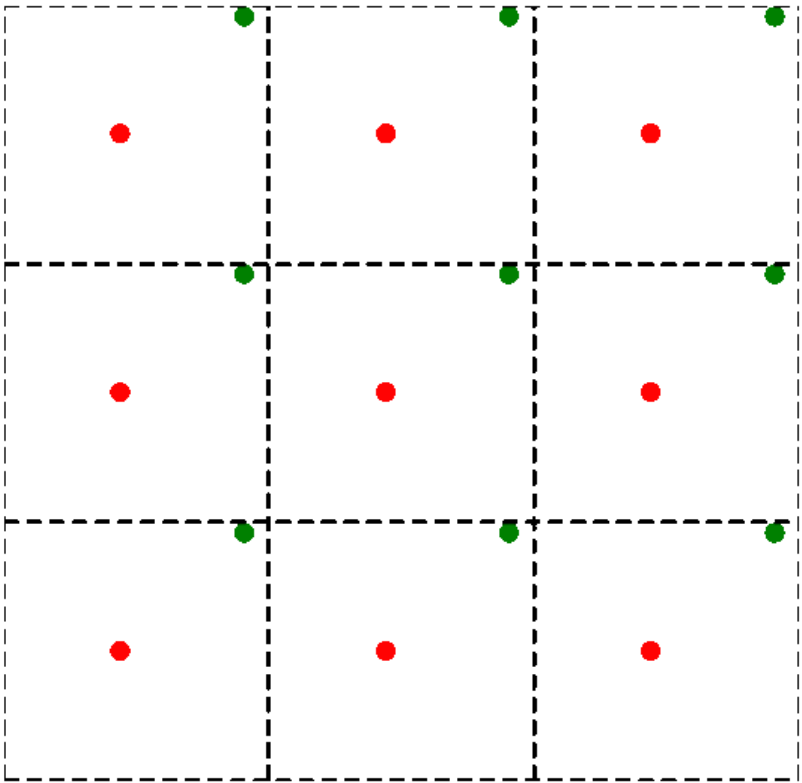
\includegraphics[width=0.55\linewidth]{images/PBC.png}
\caption{Schematic of the simulation domain with two atoms being repeated to infinity in all directions. Adapted from \cite{tudelftnotes}.}
\label{fig: PBC}
\end{figure}
}

\newcommand{\mirrorimage}{
\begin{equation}
    \mathbf{r}_\mathrm{rel}=\left(\left(\mathbf{x}_i-\mathbf{x}_j+L/2\right)\text{mod }L\right)-L/2
    \label{eqn: mirrorimage}
\end{equation}
}

\newcommand{\figmirrorimage}{
\begin{figure}[h]
\centering
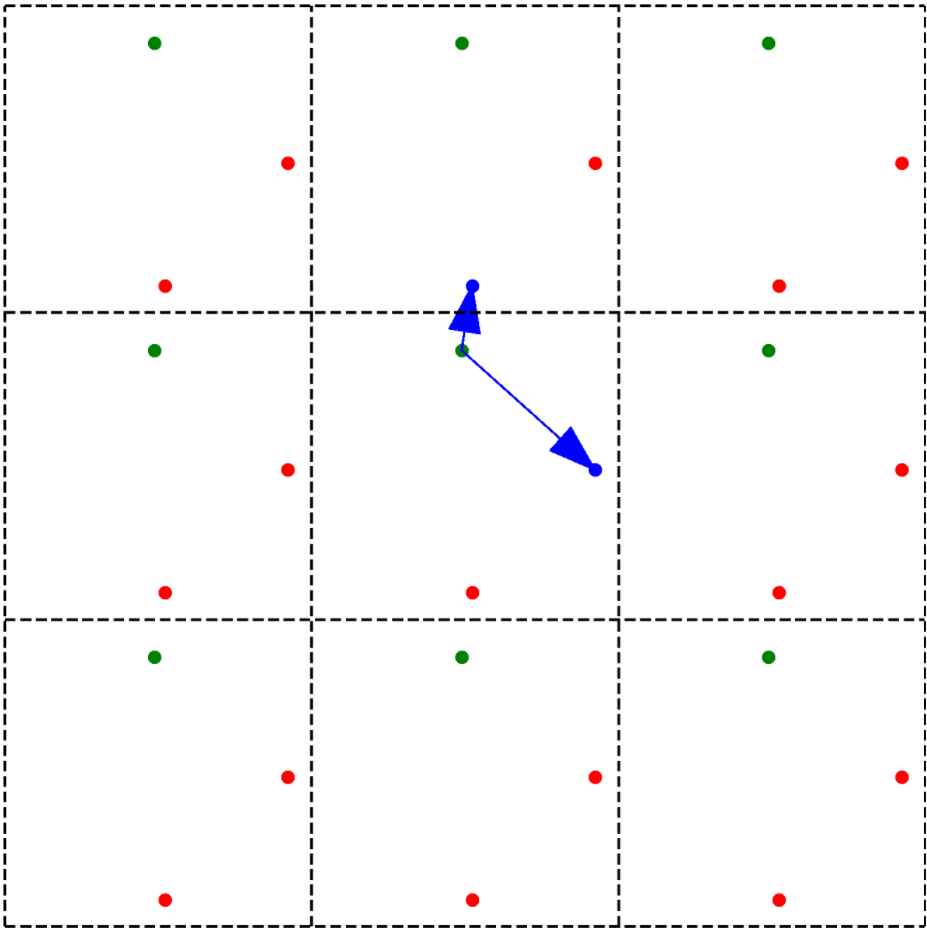
\includegraphics[width=0.55\linewidth]{images/mirrorconvention.png}
\caption{Schematic of the simulation domain with three atoms being repeated to infinity in all directions. The blue arrows denote the interaction pair that corresponds to the closest mirror image. Adapted from \cite{tudelftnotes}.}
\label{fig: mirrorimage}
\end{figure}
}

% UNUSED
\newcommand{\KEtot}{
\begin{equation}
    K_\mathrm{tot} = \sum_{i=1}^{N} \frac{mv_i^2}{2}
    \label{eqn: Total Kinetic Energy}
\end{equation}
}

%UNUSED
\newcommand{\PEtot}{
\begin{equation}
    V_\mathrm{tot} = \frac{1}{2}\sum_{i=1}^{N} V(r_{\mathrm{rel},i})
    \label{eqn: Total Potential Energy}
\end{equation}
}

\newcommand{\PEequalKE}{
\begin{equation}
E_{tot} = V_{tot} + K_{tot}, \quad \frac{dE_{tot}}{dt}=0.
\label{eq:econs}
\end{equation}
}

\newcommand{\pressure}{
\begin{equation}
\frac{\beta P}{\rho}=1-\frac{\beta}{3 N}\left\langle\frac{1}{2} \sum_{i, j} r_{i j} \frac{\partial U}{\partial r_{i j}}\right\rangle
\label{eqn: pressure}
\end{equation}
}

\newcommand{\paircorr}{
\begin{equation}
g(r)=\frac{2 V}{N(N-1)} \frac{\langle n(r)\rangle}{4 \pi r^{2} \Delta r}
\label{eqn: pair correlation function}
\end{equation}
}

\newcommand{\rescaling}{
\begin{equation}
\lambda=\sqrt{\frac{(N-1) 3 k_{B} T_D}{\sum_{i=1}^{N} m v_{i}^{2}}}
\label{eqn: rescaling}
\end{equation}
}




%%%%% REDUCED UNITS %%%%%
\newcommand{\REDUCEDLJpotential}{
\begin{equation}
    V^*(r^*_\mathrm{rel})=4\left[\left(\frac{1}{r^*_\mathrm{rel}}\right)^{12}-\left(\frac{1}{r^*_\mathrm{rel}}\right)^{6}\right]
    \label{eqn: REDUCED LJpotential}
\end{equation}
}

\newcommand{\REDUCEDLJforce}{
\begin{equation}
    \mathbf{F}^*(\mathbf{r}^*_\mathrm{rel})=-\left(\frac{24}{|\mathbf{r}^*_\mathrm{rel}|^7}-\frac{48}{|\mathbf{r}^*_\mathrm{rel}|^{13}}\right)\hat{n}
    \label{eqn: REDUCED LJforce}
\end{equation}
}

\newcommand{\REDUCEDVerletalgomod}{
\begin{equation}
\begin{aligned}
\mathbf{x}^*(t^*+\Delta t^*) &= \left( \mathbf{x}^*(t^*)+ \mathbf{v}^*(t^*)\Delta t^*+\frac{{\Delta t^*}^{2}}{2} \mathbf{F}^*(\mathbf{x}(t^*))\right)\text{mod }{L^*}  \\
\mathbf{v}^*(t^*+\Delta t^*) &=\mathbf{v}^*(t^*)+\frac{\Delta t^*}{2}(\mathbf{F}^*(\mathbf{x}^*(t^*+\Delta t^*))+\mathbf{F}^*(\mathbf{x^*}(t^*))
\end{aligned}
\label{eqn: REDUCED Verlet algorithm modulo}
\end{equation}
}

\newcommand{\REDUCEDPEequalKE}{
\begin{equation}
    E^*_\mathrm{tot}=V^*_\mathrm{tot}+K^*_\mathrm{tot}=\frac{1}{2}\sum_{i=1}^{N} V^*(r^*_{\mathrm{rel},i})+\sum_{i=1}^{N} \frac{{v^*_i}^2}{2}
    \label{eqn: REDUCED Total energy conserved}
\end{equation}
}

\newcommand{\REDUCEDpressure}{
\begin{equation}
\frac{P^*}{\rho^*T^*}=1-\frac{1}{3 N T^*}\left\langle\frac{1}{2} \sum_{i,j} r^*_{i j} \frac{\partial U^*}{\partial r^*_{ij}}\right\rangle
\label{eqn: REDUCED pressure}
\end{equation}
}

\newcommand{\REDUCEDpaircorr}{
\begin{equation}
g^*(r^*_\mathrm{rel})=\frac{2 V^*}{N(N-1)} \frac{\langle n(r^*_\mathrm{rel})\rangle}{4 \pi {r^{*}_\mathrm{rel}}^2 \Delta r^*_\mathrm{rel}}
\label{eqn: REDUCED pair correlation function}
\end{equation}
}

\newcommand{\REDUCEDrescaling}{
\begin{equation}
\lambda^*=\sqrt{\frac{(N-1) 3 T^*_D}{\sum_{i=1}^{N} v{^*_{i}}^{2}}}
\label{eqn: REDUCED rescaling}
\end{equation}
}



\newcommand{\figruntime}{
\begin{figure}[h]
\centering
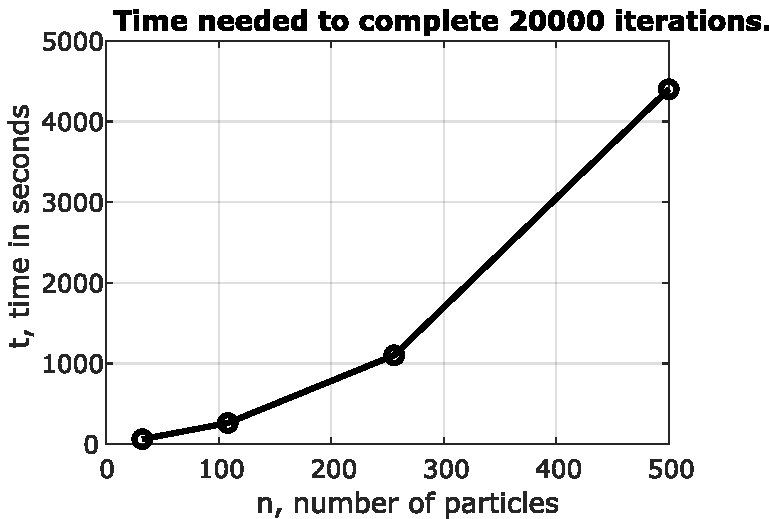
\includegraphics[width=0.75\linewidth]{images/timing.pdf}
\caption{Run-time for simulations for number of particles $n = 32, 108, 256, 500$, each with 20000 iterations. }
\label{fig: runtime}
\end{figure}
}

\usepackage{natbib}
\usepackage{braket}
\usepackage{bm}
% \usepackage[margin=3.0cm]{geometry} 
\usepackage{graphicx}
\usepackage{xcolor}
\usepackage[colorlinks = true,
            linkcolor = red,
            urlcolor  = red,
            citecolor = red,
            anchorcolor = red]{hyperref}
\hypersetup{bookmarksnumbered}

\bibliographystyle{apsrev4-2}

\begin{document}

\title{AP3082 Project 1: Molecular Dynamics}
\date{\today}

\author{Kah Jen Wo}
\affiliation{Faculty of Applied Sciences, Delft University of Technology, Delft, The Netherlands}
\author{Juan Torres}
\affiliation{Faculty of Applied Sciences, Delft University of Technology, Delft, The Netherlands}

\begin{abstract}
Molecular dynamic simulations of classical particles can be used to study the statistical behaviour of the system under different thermodynamic conditions. In this paper, we study a system of Argon atoms using the Lennard-Jones potential to model atomic interactions. We also implemented the Verlet time-evolution algorithm \cite{PhysRev.159.98} and compared our results to the original paper. A simple example with two particles is used to describe the main features of the simulation such as energy conservation. Furthermore, we investigate different phases of matter by using the pair correlation function and diffusion coefficient. Each of these observables has a characteristic behaviour for each phase of matter. Finally, we explore the limitations of our algorithm by comparing our results with the literature.
\end{abstract}
\maketitle

\section{\label{sec: Introduction}Introduction}
In a typical molecular system, there exist an enormous number of atoms such that it is not possible to analytically solve the equations of motion of the system. Then, the computation approach becomes desirable since it can simulate a large number of particles and the cost is only computational time. Several physical properties can be studied from the statistical behaviour of the system.

This approach to molecular dynamics was first conducted in 1957 by Alder and Wainwright on a hard-sphere fluid \cite{doi:10.1063/1.1743957}. The Verlet algorithm\cite{PhysRev.159.98} represented an important advance in classical molecular dynamics with respect to its predecessors such as the Euler algorithm since it was a successful model to describe the molecular dynamics of noble gases such as Argon. It is still widely used today to investigate different physical systems. Molecular dynamics has since been employed in various fields such as chemistry and physics to study phase transitions \cite{PhysRevLett.67.1886}, dynamics of polymers \cite{PhysRevA.33.3628} and ionic fluids \cite{10.1002/cphc.200700552}. 
In statistical mechanics, the properties of a time-dependent evolving microscopic molecular are calculated as an average over an ensemble of system under certain constraints. However, it requires several approximations (e.g.\ infinitely large systems) to obtain insight into the physics of the system. Using a computational approach, one can recover such features from the statistical behaviour of an arbitrary number of particles. Nevertheless, this approach presents its own challenges regarding numerical methods.

Given the importance of molecular dynamics methodology in studying complex systems, it is imperative to construct molecular dynamics simulation that is reliable and accurate. In this report, we describe the results obtained from our molecular simulation of Argon, which was implemented using \texttt{PYTHON} programming language \cite{python}. In section \ref{sec: Theoretical background}, we explain the theoretical background needed to understand the working details of the molecular dynamics simulation. In section \ref{sec: Results and Discussion}, we present the results from our simulation and expound on them. Finally, in section \ref{sec: Conclusion}, we conclude whether the results validates our molecular dynamics program.

\section{\label{sec: Theoretical background}Theoretical background}
In this section we introduce the theoretical background used for our molecular dynamics simulation. We briefly describe the particles' interaction and the evolution algorithm used. For a more detailed description of the implementation, we refer the reader to the Appendix.

\subsection{\label{subsec: Lennard-Jones fluid}Lennard-Jones fluid}
A Lennard-Jones fluid is a system of atoms governed by the pair-wise interaction potential, $V(r)$, given by \cite{tudelftnotes}:
\LJpotential
where $\epsilon$ is a measure of the interaction strength between two atoms, $\sigma$ is the characteristic distance of the interaction. Here, $r_\mathrm{rel}$ is the distance between the centre of the two particles. The first term (i.e.\ $1/r^{12}$) can be attributed to repulsive core while the second term (i.e.\ $1/r^6$) can be attributed to attractive tail. 

The Lennard-Jones force on an atom caused by another atom can be written as the negative derivative of the Lennard-Jones potential with respect to $r$:
\LJforce
where $\hat{n}$ is a unit vector along the direction of the two interacting atoms.

%With backbone of the type of dynamics defined in EQN.\ \ref{eqn: LJpotential} and EQN.\ \ref{eqn: LJforce}, we can incorporate these into the time-evolution algorithm which we will discuss in the following section.
%\textcolor{red}{INCLUDE LJ POTENTIAL PLOT!!!}
\subsection{\label{subsec: Time-evolution algorithm}Time-evolution algorithm}
The time-evolution algorithm that we are using for our molecular dynamics simulation is the velocity-Verlet algorithm because it is time reversible, sympletic and conserves volume in phase space \cite{10.1002/jcc.540150109}. This allows us to conserve the energy of the system as we will see further in this report. The evolution of position and velocity is given by \cite{PhysRev.159.98}:
\Verletalgo
where $\mathbf{F}(\mathbf{x})$ is from EQN.\ \ref{eqn: LJforce}, $\mathbf{x}$ is the relative position vector of each of the atoms with respect to other atoms, $\mathbf{v}$ is the velocity of each of the atoms, $\Delta t$ is the time-step size and $t$ is the time-step. It is important to note that $\Delta t$ must not be too big to prevent the introduction of numerical errors in the simulation. We implement dimensionless units (see \ref{subsec: Reduced Units}) to avoid numerical errors in the simulation. Since it is difficult to calculate the temperature in the initial configuration of the system, we rescale the system until it reaches a desired temperature. We consider this state as equilibrium. 

\subsection{\label{subsec: Simulation validation}Simulation Validation}
\subsubsection{\label{subsubsec: Energy Conservation}Energy Conservation}
It is known that energy must be conserved in a closed system because energy can neither be created nor destroyed. Thus, to check if our simulation is working as intended, we can check the following equality with respect to the evolving time-step.
\PEequalKE
where $K_\mathrm{tot} = \sum_{i=1}^{N} \frac{mv_i^2}{2}$ is the total kinetic energy in the system, $V_\mathrm{tot} = \frac{1}{2}\sum_{i=1}^{N} V(r_{i_\mathrm{rel}})$ is the total potential energy in the system. $N$ is the total number of atoms in the simulation domain and the $1/2$ factor in $V_\mathrm{tot}$ is introduced to prevent double-counting.


\subsubsection{\label{subsubsec: Observables}Observables}
The most commonly studied properties of microscopic molecular systems are the ones normally introduced in thermodynamics, such as pressure, $P$, or temperature, $T$, among many more. These properties are also known as "observables" because we can measure and record their values. Measuring such observables in a molecular dynamics simulation program is relatively simple, as we can use the expressions for them and compute them since we know the positions and velocities of the atoms at all time-steps. On the contrary, an experimental measurement of these quantities can be highly non-trivial.

The expression for the pressure is given as \cite{tudelftnotes}:
\pressure
where $\beta=1/k_BT$, $\rho$ is the density, and $r_{ij}$ is the distance between atom $i$ and $j$. The $1/2$ factor in the average term is introduced to prevent double-counting.

The expression for the pair correlation function is given as \cite{tudelftnotes}:
\paircorr
where $V$ is the volume of the simulation domain. The constants are the normalisation factor in the expression. $n(r)$ is a histogram of all atom pairs within a distance $[r,r+\Delta r]$, where $\Delta r$ is the bin size. Pair correlation is a reliable measure whether there is a discernible structure or pattern in a large cluster of atoms. It is used in various thermodynamics studies. In our case, however, it is a measure of how likely there is a atom at distance $r_\mathrm{rel}$ away from the observer atom.

The diffusion coefficient is a measure of how easily particle diffuse in a given system. It is well know that it has a ballistic behaviour, $D\sim t^2$, for small times since the particles do not feel the interactions of the surroundings. After this regime, it presents a diffusive behaviour like $D\sim t$. The region in which is has a ballistic motion is larger for a gas than for a liquid. For a solid it is zero. The expression for the diffusion coefficient is given by \cite{tudelftnotes}:
\begin{equation}
    D (t) = \langle \Delta x(t) \rangle = \langle [x(t=0)-x(t)]^2 \rangle.
\end{equation}

\section{\label{sec: Results and Discussion}Results and Discussion}
\subsection{\label{subsec: Two particle case}Two particle case}
\begin{figure}[h]
\centering
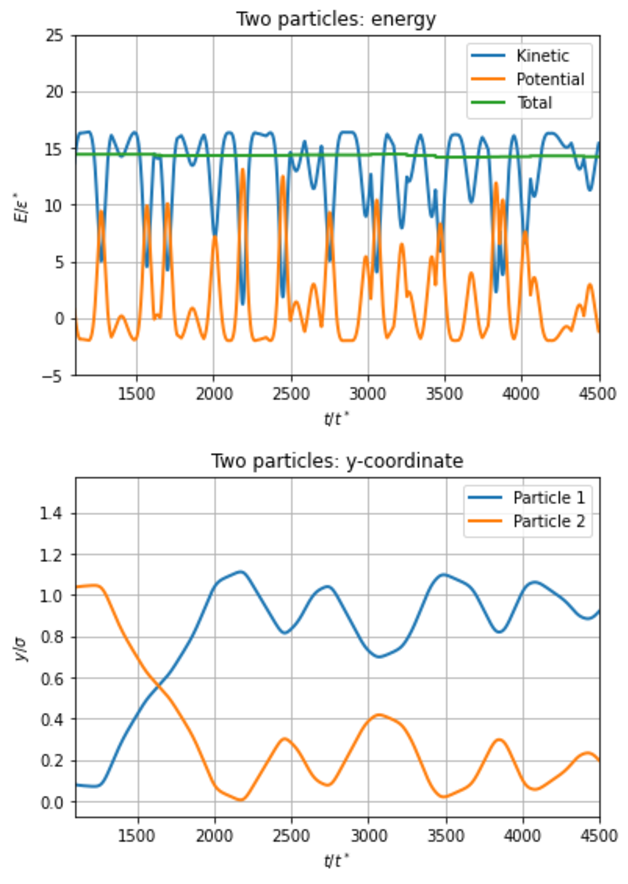
\includegraphics[width=0.85\linewidth]{images/two_particles.pdf}
\caption{Simulation of a system with two particles initialised at positions $\mathbf{r}_1=(0.1,0.5,0)$ and $\mathbf{r}_2=(0.9,0.5,0)$. The simulation domain is a square of length $L=1.5$. The system was set to reach a temperature of $T=10$. Top: Energy evolution. Bottom: $y$-coordinate evolution.}
\label{fig:two_particles}
\end{figure}
A simple harmonic oscillator can be described by considering two particles interacting via the Lennard Jones potential. This system allows us to validate the basic features of the simulation. In FIG.\ \ref{fig:two_particles} one can observe the behaviour of two particles. In the top panel one can observe the behaviour of the energy as a function of time. Once equilibrium is reached, the energy oscillates between potential and kinetic energy, and the sum of them remains constant. However, some errors can be observed around $t/t^* \sim 3250$ as little bumps in the total energy (green curve). In any case, total energy is conserved, and EQN.\ \ref{eq:econs} is satisfied. We attribute this feature to numerical errors in the integration procedure. The periodic behaviour of the system can be appreciated in the lower panel, where the $y$-coordinate of each particle is plotted with respect to time. Observe that the frequency of the oscillations is different than in the top panel. The extra frequency can found by looking at the behaviour in the $x$-coordinate.

\subsection{\label{subsec: Phases of matter}Phases of matter}

\begin{figure}[h!]
\centering
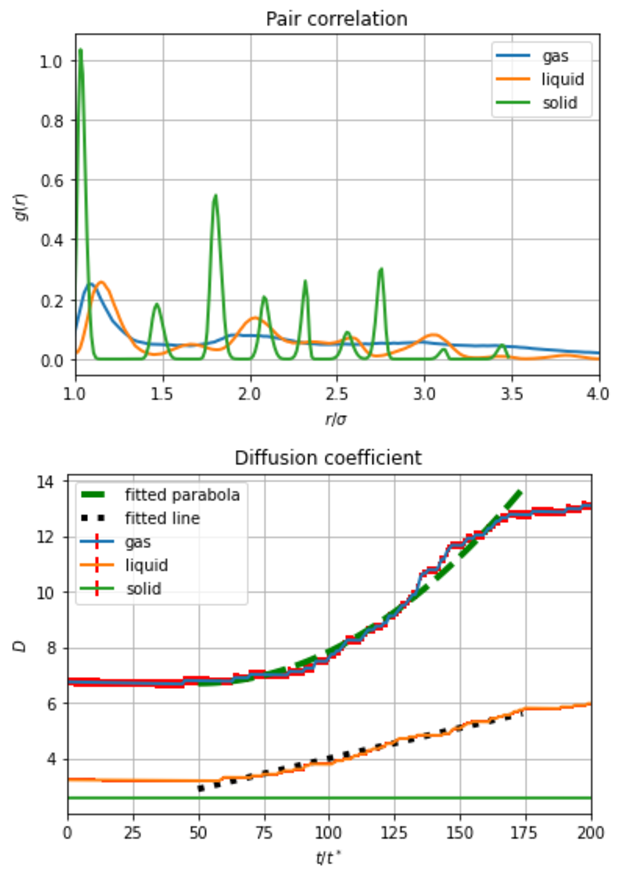
\includegraphics[width=0.85\linewidth]{images/phases.pdf}
\caption{Top: Pair correlation function with respect to distance between particles calculated for each configuration of parameters shown in Table \ref{tab:phases}. Bottom: Evolution of the Diffusion coefficient. Different behaviours can be clearly observed for each phase. Fitted line and parabola are shown to compare obtained values to theory. Fitting parameters $a$ (shift from origin) and $b$ (magnitude of $x^n$) are: $a=6.69,2.88$ and $b=4\times10^{-4},0.021$ for parabola and line, respectively. Error of gas: $0.001$. Error of liquid: $0.05$.}
\label{fig:phases}
\end{figure}
The control variables of the simulation can be specified by varying the simulation parameters. Besides of the atomic parameters, we can control the temperature and the density. These parameters are used to systematically study the behaviour of different systems corresponding to solid, liquid and gas phases. In each case, we study the diffusion constant, and the pair correlation function. These quantities have a characteristic behaviour for each situation, which will be recovered and discussed.

The initialisation of the position of the atoms must be carefully conducted. If the atoms are initialised to be too close to each other, the repulsive potential would be too large and potentially introduce simulation artefacts. We have chosen to initialise the atoms in a face-centred-cubic system where the atoms are evenly spaced. For the following simulation, we consider a unit cell of 4 atoms repeated 3 times along each coordinate. That is, $4^5$ atoms. 

The initialisation of the velocity of each of the atoms follows the a Maxwell-Boltzmann distribution (i.e.\ a Gaussian distribution) with mean $\mu=0$ and standard deviation $\varsigma=\sqrt{T^*}$. After initialising the atoms' velocities, we subtract them with the velocity of the mean of the initialised velocity such that the resulting average is 0 in every directions, keeping the atoms from drifting.

We calculate the pair correlation function and the diffusion coefficient for each phase. The values are specified in Table \ref{tab:phases}.

\begin{table}[h]
\begin{tabular}{|l|c|c|}
\hline  Phase &$\rho$ & $T$ \\
\hline Solid & 1.2 & 0.5 \\
\hline Liquid & 0.8 & 1 \\
\hline Gas & 0.3 & 3.0 \\
\hline
\end{tabular}
\caption{\label{tab:phases}Parameters corresponding to different phases of matter taken from\cite{thijsenCP}.}
\end{table}

Let us start by mentioning that we do not know a priori if these parameters indeed correspond to solid, liquid, and gas phases. We call it in this manner to distinguish between them, but we still need to verify that its behaviour correspond to what we assumed here.

The results after executing the simulation for the values of Table \ref{tab:phases} are shown in FIG.\ \ref{fig:phases}. In the top panel, we can observe the pair correlation function for each phase. The solid case (green curve) shows very distinctive peaks centred around the distances between the atoms. Here, $g(r)$ is non-zero only at the peaks, indicating that the atoms remain in its positions instead of moving around. The liquid case (orange curve) has broader peaks that overlap each other, indicating that the particles move and interact with each other. Finally, the gas case (blue curve) has a single peak at $\sigma$, and then it becomes uniform, i.e.\ correlation is equal for all distances. A common feature of these three curves is the first peak at $\sigma$ since the particles cannot come close to each other than at this distance due to core repulsion.

In the middle panel, one can observe the evolution of the diffusion coefficient for each case of Table \ref{tab:phases}. In the bottom panel of FIG.\ \ref{fig:phases} one can observe the diffusion coefficient for each case.  behaviour closely for the beginning of the simulation. Let us start observing that the solid case (green curve) has a constant behaviour over all simulating time. On the other hand, the gas and liquid cases present a non-zero behaviour. We observe that the liquid case (orange curve) has a linear behaviour, while the gas case (blue curve) has a quadratic behaviour. This result supports the idea that the system is in the corresponding phase, i.e.\ liquid and solid, since the gas behaves ballistically, while the liquid behaves diffusely.


\subsection{Statistical error in observables}
To determine the error of the values predicted by our simulation with respect to previously found values in the literature, we study the pressure under different temperatures and densities and compare it to the literature. In Table \ref{tab:pressure} one can observe the comprehensibility factor predicted by our simulation and the error with respect to the original paper of Verlet. We can observe that the values are reasonable close to the literature for small densities. For large densities, results are significantly far from literature. Nevertheless, a big difference between this simulation and the one shown in Ref.\cite{PhysRev.159.98} is the number of particles used. We used 32, while they used a value of order $10^3$. Then, it is reasonable to consider that under high densities the system has a different behaviour. 
\begin{table}[h]
\begin{tabular}{| c | c | c | c |}
\hline  $\rho$ &$T$ & $\beta P/\rho$ & Error \\
\hline $0.88$ & $1.095$ & $0.9548\pm 0.0001$ & $72.58\%$\\
\hline $0.85$ & $2.889$ & $2.4579\pm0.0003$ & $46.65\%$\\
\hline $0.75$ & $2.849$ & $2.1373\pm0.0003$ & $31.06\%$\\
\hline $0.65$ & $1.585$ & $1.0275\pm0.0002$ & $17.84\%$\\
\hline $0.55$ & $2.645$ & $1.453\pm0.0002$ & $10.86\%$\\
\hline $0.45$ & $4.625$ & $2.0805\pm0.0001$ & $23.81\%$\\
\hline
\end{tabular}
\caption{\label{tab:pressure}Simulation of 32 particles for different values of density and temperature. Quantities are in dimensionless units. Error in third column was calculated using autocorrelation function method.\cite{tudelftnotes} Last column corresponds to the error with respect to original values from Verlet paper\cite{PhysRev.159.98}.}
\end{table}

\section{\label{sec: Conclusion}Conclusion}
In summary, we simulated a simple example with two particles as shown in section \ref{subsec: Two particle case} and found that the total energy is indeed conserved according to EQN.\ \ref{eqn: REDUCED Total energy conserved} with negligible numerical integration errors. Furthermore, we also analysed for gas, solid, and liquid phase of matter in section \ref{subsec: Phases of matter} by measuring several properties, namely, pair correlation function and diffusion coefficient. We found the expected behaviour for the physical quantities for each phase and we concluded that the simulation described the different phases of matter successfully. However, we did not explore phase transitions. Additionally, we recovered values from the literature for the compressibility within a reasonable error range. We attribute it to the fact that we only simulated $n=32$ particles, while the original paper simulated around 10k. The error is the largest for high densities.

\section{\label{sec: Acknowledgements}Acknowledgements}
This work is part of the course AP3082 Computational Physics supported by the Delft University of Technology.

% \section*{Appendix}
\appendix\label{appendix}
\section{\label{subsec: Periodic Boundary Condition}Periodic Boundary Condition}
A study of the Lennard-Jones fluid system would only be meaningful if we simulate large number of atoms. However, that is not feasible due to the computational constraints such as run-time and memory. One way to circumvent this is by introducing periodic boundary condition (PBC), which is useful in emulating a system of infinite particles. To incorporate PBC in our simulation, we just have to introduce modulo to the position part of EQN.\ \ref{eqn: Verlet algorithm} as shown while the velocity part stays the same:
\Verletalgomod
where $L$ is the length of the simulation domain in the direction of $\mathbf{x}$. The introduction of the modulo term allows for the atoms to reappear from the opposite side of the simulation domain if they go over one side. It is also mathematically equivalent to the simulation domain being replicated in all directions as shown in FIG.\ \ref{fig: PBC}.
\figPBC

\section{\label{subsec: Minimal Mirror Convention}Minimal Mirror Convention}
In a simulation domain with periodic boundary condition, each particle in it has infinitely many neighbours due to the simulation domain being repeated to infinity. Computing the distance between infinitely many pairs of particles is impossible. However, there exists an ingenious way to solve this problem: minimal image convention \cite{tudelftnotes}. In FIG.\ \ref{fig: mirrorimage}, we illustrate this convention in a system of three atoms in the simulation domain.
\figmirrorimage

In this convention, we consider only the interaction between particle pairs in the nearest repeating simulation domain image, including the original simulation domain.
\mirrorimage
By incorporating EQN.\ \ref{eqn: mirrorimage} into the Verlet algorithm with PBC (i.e.\ EQN.\ \ref{eqn: Verlet algorithm modulo}), we arrive at the full algorithm for running our molecular dynamics simulations program.

\section{\label{subsec: Rescaling}Rescaling}
To study a system at a desired temperature $T_D$, we cannot just initialise the system at $T_D$. This is because the system would evolve and equilibrate the a configuration with a different temperature. Thus, we need to externally force the kinetic energy of the system to that of the desired temperature $T_D$ after letting it equilibrate for a while.

The rescaling factor is given as \cite{tudelftnotes}:
\rescaling
With this, we can perform the indirect rescaling of the kinetic energy by changing the velocities of the atoms as such: $\mathbf{v}_i\rightarrow\lambda\mathbf{v}_i$. After several rescalings, we should arrive at the desired temperature and we can study the observables at the intended temperature.

\section{\label{subsec: Reduced Units}Reduced Units}
Reduced units or dimensionless units is important because it offers several advantages compared to using the default units:
\begin{itemize}
\item Less number of constants that need to be keep track of.
\item Simplified expressions improve readability.
\item Intuition into the appropriate length/time scales in a given system.
\end{itemize}
In TABLE.\ \ref{tab: reduced units}, we see the conversion between the default units and reduced units.
\tabreducedunits

Using TABLE.\ \ref{tab: reduced units}, we re-derive the relevant expression below in the previous sections.

The Lennard-Jones potential (EQN.\ \ref{eqn: LJpotential}) becomes:
\REDUCEDLJpotential
The force due to Lennard-Jones potential (EQN.\ \ref{eqn: LJforce}) becomes:
\REDUCEDLJforce
The Verlet algorithm (EQN.\ \ref{eqn: Verlet algorithm modulo}) becomes:
\REDUCEDVerletalgomod
The kinetic and potential energy become (EQN.\ \ref{eq:econs}) becomes:
\REDUCEDPEequalKE
The pressure (EQN.\ \ref{eqn: pressure}) becomes:
\REDUCEDpressure
The pair-correlation function (EQN.\ \ref{eqn: pair correlation function}) becomes:
\REDUCEDpaircorr
The rescaling factor (EQN.\ \ref{eqn: rescaling}) becomes:
\REDUCEDrescaling
We will use these new expressions in our molecular dynamics simulation.

\section{\label{subsec: Run-time}Run-time}
To analyse the running time of our simulation program, we ran simulations for different number of particles as shown in FIG.\ \ref{fig: runtime}.
\figruntime
We see that the time needed to complete 20000 iterations of the molecular dynamics evolution grows exponentially. At $n=500$, we already need $\sim{4500}$ seconds (i.e.\ 1.25 hours). From this we know that the computation time using our program for higher $n$ is going to be much larger than 1.25 hours. To study the phase diagram of the of a given system, we need to run multiple simulation runs each with many iterations. Thus, the program at its current state is not sufficient to be used to carry state-of-the-art molecular dynamics research.


% \nocite{*}
\bibliography{references}% Produces the bibliography via BibTeX.
\end{document}